\section{3D-Laplace}
The previous chapter focused on describing the use of 2-dimensional noise on geographical data.
This approach has recently been extended to support 3-dimensional data, which benefits indoor navigation \citep{9646489}.
The method is similar to the 2D approach but includes the azimuth angle $\psi$, in addition to the polar angle $\theta$ and radius $r$.

\subsection{Geo-indistinguishability}
To establish the same privacy guarantees for 3-dimensional data as for 2-dimensional data, the original equation \ref{algo:2d-geo-indistinguishability} is extended \citep{9646489}.
\begin{equation}
  K(x_1)(z) \le e^{\epsilon * d_3(x_1, x_2)} K(x_2)(z)
  \label{algo:3d-geo-indistinguishability}
\end{equation}
Where $x_1$ and $x_2$ are two real data points in the same dataset $X$.
%The more $x_1$ and $x_2$ are similar, the more the perturbed location distributions $K(x_1)(z)$ and $K(x_2)(z)$ need to be similar.
\subsection{Spherical Laplace}
The implementation of Min et al. projects the dimensions onto a sphere instead of a circle \citep{9646489}.
This sphere is a unit sphere calculated with a radius of 1.
Based on this sphere the polar angle $\theta$ and azimuth angle $\psi$ are randomly calculated. \newline
\textbf{Calculating $\theta$ and $\psi$}: Both are drawn from the unit sphere using the following equations:
\begin{equation}
  \theta = \frac{1}{\pi}
\end{equation}
\begin{equation}
  \psi = \frac{1}{2\pi}
\end{equation}
The tuple $U = (\theta, \psi)$ is randomly selected based on the uniform distribution of the unit sphere \citep{9646489}. \newline
\textbf{Calculating $r$}: The radius $r$ (distance from the center) is calculated using the following equation:
\begin{equation}
  r = \frac{1}{2}\epsilon^3 * r^2 * e^{-\epsilon * r}
  \label{eq:3d-laplace-r}
\end{equation}
Where the gamma scale is the same as for 2D-Laplace, but with a shape of 3 instead of 2.
The noise is added to the original location $x$ to obtain the perturbed location $z = x + U*r$.
A clear example of the noise that is generated by this method is shown in figure \ref{fig:3d-laplace-noise}.
\begin{figure}
  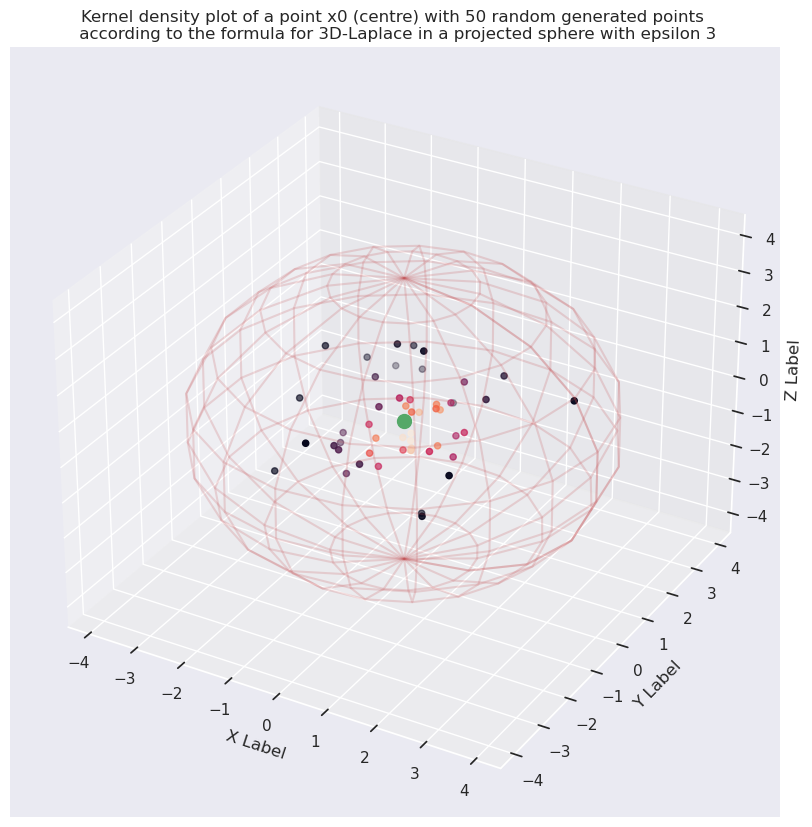
\includegraphics[width=0.6\textwidth]{TheorethicalFramework/ND-Laplace/Images/3d_laplace_noise.png}
  \caption{50 random noise samples generated around point $x_0$ (green dot) using the 3D-Laplace noise method \citep{9646489} plotted on a sphere.}
  \label{fig:3d-laplace-noise}
\end{figure}
Finally, we convert this to the Cartesian coordinate system to obtain the final location $z$:
\begin{align*}
  z_x = r * \sin(\theta) * \sin(\psi) \\
  z_y = r * \sin(\theta) * \cos(\psi) \\
  z_z = r * \cos(\theta)
\end{align*}
This is also visualized in figure \ref{fig:3d-laplace}.
\begin{figure}
  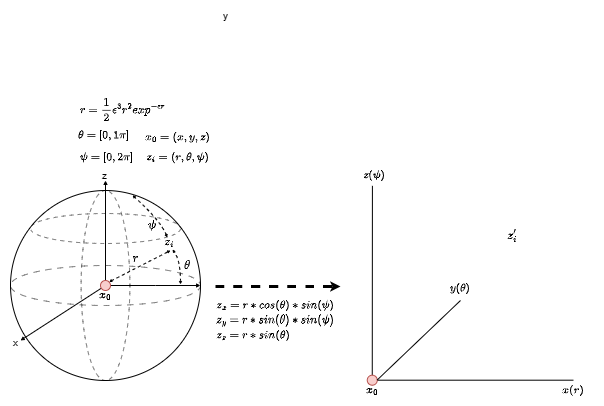
\includegraphics[width=0.8\textwidth]{TheorethicalFramework/ND-Laplace/Images/3d_laplace.png}
  \caption{3D-Laplace noise distribution according to the method proposed by Min et al. \citep{9646489}}
  \label{fig:3d-laplace}
\end{figure}
\newpage
\subsection{Truncation}
As with the 2D-Laplace method, the 3D-Laplace method also has a truncation method.
This truncation method is also based on the same method as the 2D-Laplace method.
Instead of a plane grid, a cuboid grid is used for 3-dimensional space.
This also remaps the noise to the closest grid point or existing point.
To demonstrate this, we plotted example data points on a 3-dimensional grid in figure \ref{fig:3d-laplace-example}.
\begin{figure} [ht]
  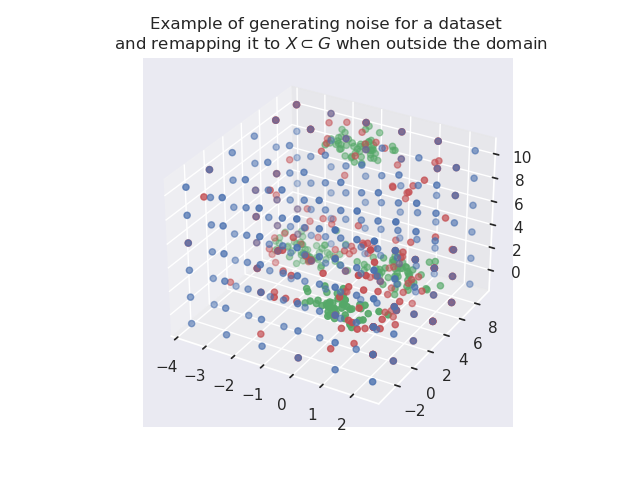
\includegraphics{TheorethicalFramework/ND-Laplace/Images/example_3d_laplace.png}
  \caption{Applying 3-dimensional noise with $\epsilon = 1$ (red dots) to a dataset $X$ (green dots). Demonstrating remapping to the closest grid point (blue) or $X$.}
  \label{fig:3d-laplace-example}
\end{figure}